

\section{MIP Model}
The MIP formulation was developed with Pyomo, a Python library for writing solver-independent models.
Two models were developed: a base version composed of a 4d array with symmetry breaking and implied constraints, and a better one, optimizing the number of variables featuring circle matching.

\subsection{Variables}
Let $n$ be the number of teams. We define the sets of teams, weeks, and periods per week as
\[
T = \{0, \dots, n-1\}, \quad W = \{0, \dots, n-2\}, \quad P = \left\{0, \dots, \frac{n}{2} - 1\right\}.
\]
Let $wp = (w,p)$ be the week/period slot $w,p$;
let $m_{i,j} = (i,j)$ be the match played by team $i,j$ with $i<j$:
\[
WP = (\{0, \dots, n-2\},\{0, \dots, \frac{n}{2} - 1\}), \quad M = (\{0, \dots, n-1\},\{0, \dots, n-1\})
\]

\subsubsection*{Decision Variables}
To encode the STS problem, two variables were used:
\begin{enumerate}
\item $\text{\textbf{Y}}[wp,m] \in \{0,1\}$ \quad $\forall wp \in (W,P)$, $\forall m_{i,j} \in \{T,T\}$ with $i<j$.
\item $\text{\textbf{H}}[i]$ $\in \{0,1\}$ \quad $\forall i \in T$. \\ 
\end{enumerate}
\subsubsection*{Implied Variables}
The implied constraint needs a variable \textbf{Q}$[i,p] \in [0,1]$ that keeps track of which team played on which period.

\subsection{Objective Function}
\paragraph{Variables}
In order to minimize the maximum imbalance, we need 3 extra variables:
\begin{enumerate}
\item \textbf{Home}$[i]$ $\in [0,n-1]$: the number of home matches played by team i
\item \textbf{Away}$[i]$ $\in [0,n-1]$: the number of away matches played by team i
\item \textbf{Z} $ \in [0,n-1]$: the maximum imbalance
\end{enumerate}

\paragraph{Constraints}
With circle matching we get a matrix:
\[
\text{presolved[w,i,j] = }
\begin{cases}
    \text{1 \quad if the match (i,j) is scheduled for week w}\\
    \text{0 \quad o.w.}
\end{cases}
\]
To take advantage of the precomputed matching schedule, we enforce:
\[\forall w \in W, \forall p \in P, \forall m \in M, m = (i,j): \textbf{Y}[(w,p),m] \leq \text{presolved}[w,i,j]\]


\subsection{Constraints}
In this particular model the addition of symmetry breaking constraints did not improve the results, as circle matching already breaks most of the symmetries, and the addition of other constraints only increased the model weight.

\begin{enumerate}
\item \textbf{one match per w/p slot}: 
\[\forall wp \in WP: \quad\sum_{m \in M}^{m} \textbf{Y}[wp, m] = 1\]
\item \textbf{one w/p slot per match}: 
\[\forall m \in M: \quad\sum_{wp \in WP}^{wp} \textbf{Y}[wp, m] = 1\]
\item \textbf{at most 2 matches in the same period}: 
\[
\forall p \in P, \forall k \in T:
\sum_{w \in W}^{w}\sum_{j \in \{k+1\dots n\}}^{j} \textbf{Y}[(w,p), (k,j)] + 
\sum_{w \in W}^{w}\sum_{i \in \{0\dots k\}}^{i} \textbf{Y}[(w,p), (i,k)] <= 2
\]
\end{enumerate}

\subsubsection*{Constraints for efficiency}
Especially useful in an optimization environment, this constraint aims to spread the matches of a team in different periods over the scheduling, to get a more balanced result. It also help with symmetry breaking.
\[
    \forall p \in P, \forall i \in T: \quad 2 \textbf{Q}[i,p] \geq 
    \sum_{w \in W}^{w}\sum_{j \in \{i+1\dots n\}}^{j} \textbf{Y}[(w,p), (i,j)] + 
    \sum_{w \in W}^{w}\sum_{j \in \{0\dots i\}}^{j} \textbf{Y}[(w,p), (j,i)]
\]
\[
    \forall i \in T: \quad \sum{p \in P}^p \textbf{Q}[i,p] \geq ceil((n-1)/2)
\]

\subsubsection*{Objective constraints}
\begin{enumerate}
    \item \textbf{home games}: 
\[\forall i \in T: \quad Home[i] = \sum_{j \in T}^{j} \textbf{H}[(i,j)] + \sum_{j \in T}^{j} (1- \textbf{H}[(j,i)]) \quad \text{with $i < j$}\]
    \item \textbf{away games}: 
\[\forall i \in T: \quad Home[i] = \sum_{j \in T}^{j} (1- \textbf{H}[(i,j)]) + \sum_{j \in T}^{j} \textbf{H}[(j,i)] \quad \text{with $i < j$}\]
    \item \textbf{max imbalance}:
\[\forall i \in T: \quad  \textbf{Home}[i] - \textbf{Away}[i] \leq \textbf{Z} \bigwedge
\forall i \in T: \quad  \textbf{Away}[i] - \textbf{Home}[i] \leq \textbf{Z} \]

\end{enumerate}

\subsection{4d array model}
The simplest possible implementation of the STS problem, developed only for comparison as it is not nearly as efficient as the previous one.
The only decision variable is X, a 4d array n-1 x n/2 x n x n of binary values, where each cell represents a match, described as a combination of week, period, team1 and team2. The first team is the one playing home.
The constraints, apart from the necessary ones, include two symmetry-breaking constraints and two implied constraints.
The optimization is performed in the same way as in the previous model.

The results were obtained by running the models for 3 different solvers: Cbc, Glpk and Guroby. Cbc and Glpk are open source solvers while Gurobi is proprietary, used under an academic license.

\subsection{Validation}
The model was implemented in Python using Pyomo 6.9.2. 
The results were obtained by running the models for 3 different solvers:
\begin{enumerate}
    \item \textbf{Glpk}: open-source GNU MIP and LP solver, works well for small instances, but does not scale well.
    \item \textbf{Cbc}: open-source solver based on CLP, thanks to its advanced heuristics and cutting planes performs well even on larger problems.
    \item \textbf{Gurobi}: a commercial solver, under an academic license, which is required to reproduce its results.
\end{enumerate}

\subsubsection{Experimental Results}
We tested the MIP formulation in all the combinations allowed by the model. Here are some of the most interesting results, for a more complete list see the $/res$ folder of the project work.
It might by newsworthy to point out that 

\begin{figure}[H]
    \label{fig:mip1}
    \centering
    \begin{subfigure}{\linewidth}
        \centering
        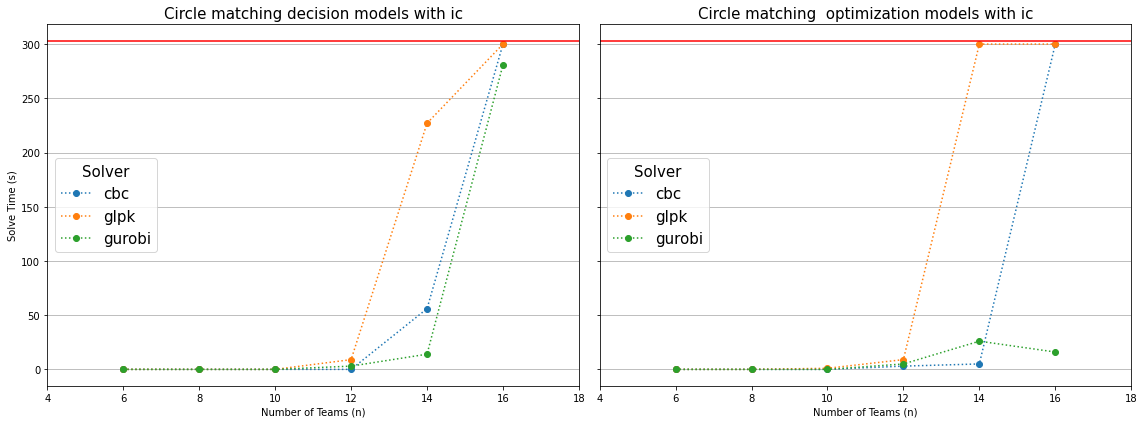
\includegraphics[width=\linewidth]{imgs/plot1.png}
        \caption{Decision vs Optimization}
    \end{subfigure}
\end{figure}

\paragraph{Decision version}
The decision version of the problem, counterintuitively, required on average more time to solve, as shown in figure \ref{fig:mip1}. This fact is explained by the nature of the search in MIP, that focus on the objective more that the constraints.
The constraints added for the sole purpose of efficiency were not only useless, but even detrimental.

\begin{table}[H]
    \centering
    \begin{tabular}{|c|c|c|c|}
    \hline
        \textbf{n} &  \textbf{Model} & \textbf{Solver} & \textbf{Time} \\
    \hline
         8 & 4D & Glpk & 1s \\
         10 & 4D & Glpk & 300s \\
         10 & 4D & Cbc & 5s \\
         12 & 4D & Cbc & 300s \\
         12 & 4D & Gurobi & 23s \\
         12 & CM & Glpk & 14s \\
         12 & CM & Cbc & 11s \\
    \hline
    \end{tabular}
    \begin{tabular}{|c|c|c|c|}
    \hline
        \textbf{n} &  \textbf{Model} & \textbf{Solver} & \textbf{Time} \\
    \hline
        12 & CM & Gurobi & 2s \\
         14 & 4D & Gurobi & 24s \\
         14 & CM & Glpk & 300s \\
         14 & CM & Cbc & 27s \\
         14 & CM & Gurobi & 36s \\
         16 & CM & Cbc & 300s \\
         16 & CM & Gurobi & 72s \\
    \hline
    \end{tabular}
    \caption{Results for the decision problem}
    \text{\small{All with efficiency constraints off}}
    \label{tab:mip1}
\end{table}

\paragraph{Optimization version}
In both versions of the problem the simpler model it significantly outperformed by the circle matching approach, as expected.
The results obtained by the different solvers are not surprising either: for both models and versions, Glpk was the worse performing while Gurobi was the best, followed by Cbc with with a short lead.

%table2
\begin{table}[H]
    \centering
    \begin{tabular}{|c|c|c|c|c|}
    \hline
        \textbf{n} &  \textbf{Model} & \textbf{Solver} & \textbf{Time} & \textbf{Opt} \\
    \hline
         10 & 4D & Cbc & 298s & no \\
         10 & 4D & Glpk & 44s & yes \\
         10 & 4D & Gurobi & 5s & yes \\
         12 & 4D & Cbc/Glpk & 300s & no \\
         12 & CM & Cbc & 3s & yes \\
         12 & CM & Glpk & 9s & yes \\
    \hline
    \end{tabular}
    \begin{tabular}{|c|c|c|c|c|}
    \hline
        \textbf{n} &  \textbf{Model} & \textbf{Solver} & \textbf{Time} & \textbf{Opt} \\
    \hline
         12 & CM & Gurobi & 5s & yes \\
         14 & CM & Cbc & 5s & yes \\
         14 & CM & Glpk & 300s & no \\
         14 & CM & Gurobi & 26s & yes \\
         16 & CM & Cbc & 300s & no \\
         16 & CM & Gurobi & 16s & yes \\
    \hline
    \end{tabular}
    \caption{Results for the optimization problem}
    \text{\small{All with efficiency constraints on}}
    \label{tab:mip1}
\end{table}